% Options for packages loaded elsewhere
\PassOptionsToPackage{unicode}{hyperref}
\PassOptionsToPackage{hyphens}{url}
\PassOptionsToPackage{dvipsnames,svgnames,x11names}{xcolor}
%
\documentclass[
  letterpaper,
  DIV=11,
  numbers=noendperiod]{scrartcl}

\usepackage{amsmath,amssymb}
\usepackage{lmodern}
\usepackage{iftex}
\ifPDFTeX
  \usepackage[T1]{fontenc}
  \usepackage[utf8]{inputenc}
  \usepackage{textcomp} % provide euro and other symbols
\else % if luatex or xetex
  \usepackage{unicode-math}
  \defaultfontfeatures{Scale=MatchLowercase}
  \defaultfontfeatures[\rmfamily]{Ligatures=TeX,Scale=1}
\fi
% Use upquote if available, for straight quotes in verbatim environments
\IfFileExists{upquote.sty}{\usepackage{upquote}}{}
\IfFileExists{microtype.sty}{% use microtype if available
  \usepackage[]{microtype}
  \UseMicrotypeSet[protrusion]{basicmath} % disable protrusion for tt fonts
}{}
\makeatletter
\@ifundefined{KOMAClassName}{% if non-KOMA class
  \IfFileExists{parskip.sty}{%
    \usepackage{parskip}
  }{% else
    \setlength{\parindent}{0pt}
    \setlength{\parskip}{6pt plus 2pt minus 1pt}}
}{% if KOMA class
  \KOMAoptions{parskip=half}}
\makeatother
\usepackage{xcolor}
\setlength{\emergencystretch}{3em} % prevent overfull lines
\setcounter{secnumdepth}{-\maxdimen} % remove section numbering
% Make \paragraph and \subparagraph free-standing
\ifx\paragraph\undefined\else
  \let\oldparagraph\paragraph
  \renewcommand{\paragraph}[1]{\oldparagraph{#1}\mbox{}}
\fi
\ifx\subparagraph\undefined\else
  \let\oldsubparagraph\subparagraph
  \renewcommand{\subparagraph}[1]{\oldsubparagraph{#1}\mbox{}}
\fi

\usepackage{color}
\usepackage{fancyvrb}
\newcommand{\VerbBar}{|}
\newcommand{\VERB}{\Verb[commandchars=\\\{\}]}
\DefineVerbatimEnvironment{Highlighting}{Verbatim}{commandchars=\\\{\}}
% Add ',fontsize=\small' for more characters per line
\usepackage{framed}
\definecolor{shadecolor}{RGB}{241,243,245}
\newenvironment{Shaded}{\begin{snugshade}}{\end{snugshade}}
\newcommand{\AlertTok}[1]{\textcolor[rgb]{0.68,0.00,0.00}{#1}}
\newcommand{\AnnotationTok}[1]{\textcolor[rgb]{0.37,0.37,0.37}{#1}}
\newcommand{\AttributeTok}[1]{\textcolor[rgb]{0.40,0.45,0.13}{#1}}
\newcommand{\BaseNTok}[1]{\textcolor[rgb]{0.68,0.00,0.00}{#1}}
\newcommand{\BuiltInTok}[1]{\textcolor[rgb]{0.00,0.23,0.31}{#1}}
\newcommand{\CharTok}[1]{\textcolor[rgb]{0.13,0.47,0.30}{#1}}
\newcommand{\CommentTok}[1]{\textcolor[rgb]{0.37,0.37,0.37}{#1}}
\newcommand{\CommentVarTok}[1]{\textcolor[rgb]{0.37,0.37,0.37}{\textit{#1}}}
\newcommand{\ConstantTok}[1]{\textcolor[rgb]{0.56,0.35,0.01}{#1}}
\newcommand{\ControlFlowTok}[1]{\textcolor[rgb]{0.00,0.23,0.31}{#1}}
\newcommand{\DataTypeTok}[1]{\textcolor[rgb]{0.68,0.00,0.00}{#1}}
\newcommand{\DecValTok}[1]{\textcolor[rgb]{0.68,0.00,0.00}{#1}}
\newcommand{\DocumentationTok}[1]{\textcolor[rgb]{0.37,0.37,0.37}{\textit{#1}}}
\newcommand{\ErrorTok}[1]{\textcolor[rgb]{0.68,0.00,0.00}{#1}}
\newcommand{\ExtensionTok}[1]{\textcolor[rgb]{0.00,0.23,0.31}{#1}}
\newcommand{\FloatTok}[1]{\textcolor[rgb]{0.68,0.00,0.00}{#1}}
\newcommand{\FunctionTok}[1]{\textcolor[rgb]{0.28,0.35,0.67}{#1}}
\newcommand{\ImportTok}[1]{\textcolor[rgb]{0.00,0.46,0.62}{#1}}
\newcommand{\InformationTok}[1]{\textcolor[rgb]{0.37,0.37,0.37}{#1}}
\newcommand{\KeywordTok}[1]{\textcolor[rgb]{0.00,0.23,0.31}{#1}}
\newcommand{\NormalTok}[1]{\textcolor[rgb]{0.00,0.23,0.31}{#1}}
\newcommand{\OperatorTok}[1]{\textcolor[rgb]{0.37,0.37,0.37}{#1}}
\newcommand{\OtherTok}[1]{\textcolor[rgb]{0.00,0.23,0.31}{#1}}
\newcommand{\PreprocessorTok}[1]{\textcolor[rgb]{0.68,0.00,0.00}{#1}}
\newcommand{\RegionMarkerTok}[1]{\textcolor[rgb]{0.00,0.23,0.31}{#1}}
\newcommand{\SpecialCharTok}[1]{\textcolor[rgb]{0.37,0.37,0.37}{#1}}
\newcommand{\SpecialStringTok}[1]{\textcolor[rgb]{0.13,0.47,0.30}{#1}}
\newcommand{\StringTok}[1]{\textcolor[rgb]{0.13,0.47,0.30}{#1}}
\newcommand{\VariableTok}[1]{\textcolor[rgb]{0.07,0.07,0.07}{#1}}
\newcommand{\VerbatimStringTok}[1]{\textcolor[rgb]{0.13,0.47,0.30}{#1}}
\newcommand{\WarningTok}[1]{\textcolor[rgb]{0.37,0.37,0.37}{\textit{#1}}}

\providecommand{\tightlist}{%
  \setlength{\itemsep}{0pt}\setlength{\parskip}{0pt}}\usepackage{longtable,booktabs,array}
\usepackage{calc} % for calculating minipage widths
% Correct order of tables after \paragraph or \subparagraph
\usepackage{etoolbox}
\makeatletter
\patchcmd\longtable{\par}{\if@noskipsec\mbox{}\fi\par}{}{}
\makeatother
% Allow footnotes in longtable head/foot
\IfFileExists{footnotehyper.sty}{\usepackage{footnotehyper}}{\usepackage{footnote}}
\makesavenoteenv{longtable}
\usepackage{graphicx}
\makeatletter
\def\maxwidth{\ifdim\Gin@nat@width>\linewidth\linewidth\else\Gin@nat@width\fi}
\def\maxheight{\ifdim\Gin@nat@height>\textheight\textheight\else\Gin@nat@height\fi}
\makeatother
% Scale images if necessary, so that they will not overflow the page
% margins by default, and it is still possible to overwrite the defaults
% using explicit options in \includegraphics[width, height, ...]{}
\setkeys{Gin}{width=\maxwidth,height=\maxheight,keepaspectratio}
% Set default figure placement to htbp
\makeatletter
\def\fps@figure{htbp}
\makeatother

\KOMAoption{captions}{tableheading}
\makeatletter
\makeatother
\makeatletter
\makeatother
\makeatletter
\@ifpackageloaded{caption}{}{\usepackage{caption}}
\AtBeginDocument{%
\ifdefined\contentsname
  \renewcommand*\contentsname{Table of contents}
\else
  \newcommand\contentsname{Table of contents}
\fi
\ifdefined\listfigurename
  \renewcommand*\listfigurename{List of Figures}
\else
  \newcommand\listfigurename{List of Figures}
\fi
\ifdefined\listtablename
  \renewcommand*\listtablename{List of Tables}
\else
  \newcommand\listtablename{List of Tables}
\fi
\ifdefined\figurename
  \renewcommand*\figurename{Figure}
\else
  \newcommand\figurename{Figure}
\fi
\ifdefined\tablename
  \renewcommand*\tablename{Table}
\else
  \newcommand\tablename{Table}
\fi
}
\@ifpackageloaded{float}{}{\usepackage{float}}
\floatstyle{ruled}
\@ifundefined{c@chapter}{\newfloat{codelisting}{h}{lop}}{\newfloat{codelisting}{h}{lop}[chapter]}
\floatname{codelisting}{Listing}
\newcommand*\listoflistings{\listof{codelisting}{List of Listings}}
\makeatother
\makeatletter
\@ifpackageloaded{caption}{}{\usepackage{caption}}
\@ifpackageloaded{subcaption}{}{\usepackage{subcaption}}
\makeatother
\makeatletter
\@ifpackageloaded{tcolorbox}{}{\usepackage[many]{tcolorbox}}
\makeatother
\makeatletter
\@ifundefined{shadecolor}{\definecolor{shadecolor}{rgb}{.97, .97, .97}}
\makeatother
\makeatletter
\makeatother
\ifLuaTeX
  \usepackage{selnolig}  % disable illegal ligatures
\fi
\IfFileExists{bookmark.sty}{\usepackage{bookmark}}{\usepackage{hyperref}}
\IfFileExists{xurl.sty}{\usepackage{xurl}}{} % add URL line breaks if available
\urlstyle{same} % disable monospaced font for URLs
\hypersetup{
  pdftitle={Vitesse de synthèse},
  pdfauthor={Sophie D., François M., Karen P.},
  colorlinks=true,
  linkcolor={blue},
  filecolor={Maroon},
  citecolor={Blue},
  urlcolor={Blue},
  pdfcreator={LaTeX via pandoc}}

\title{Vitesse de synthèse}
\author{Sophie D., François M., Karen P.}
\date{}

\begin{document}
\maketitle
\ifdefined\Shaded\renewenvironment{Shaded}{\begin{tcolorbox}[interior hidden, sharp corners, enhanced, borderline west={3pt}{0pt}{shadecolor}, breakable, boxrule=0pt, frame hidden]}{\end{tcolorbox}}\fi

\hypertarget{contexte}{%
\subsection{Contexte}\label{contexte}}

On s'intéresse à des images composées de points verts et rouges, chaque
point correspondant à un bout précis de l'ADN.

Quand ces bouts d'ADN ont été lus, la particule s'éteint.

Cependant, ces particuliers s'éteignent aussi même sans avoir été lus
(parce que éclairés trop longtemps par exemple).

On note \(i\) un bout d'ADN représenté par un point vert et un point
rouge. Soit \(n\) leur nombre.

Après traitement d'image, on peut observer sur un intervalle de temps
donné \([T_0, T]\), les instants de mort
\[(T_i^R, T^V_i)_{i=1,\dots n}.\]

Deux processus de morts sont à l'oeuvre et se cumulent:

\begin{itemize}
\item
  Mort naturelle (dûe à la durée de l'éclairage)
\item
  Mort par lecture
\end{itemize}

Pour toute entité \(i\), soit \(U_i^{R}\) l'instant de mort naturelle de
la particule \(R\) (idem pour \(V\)) et soit \(V_i^{R}\) sa mort par
lecture.

Alors

\[
\begin{array}{ccl}
T_i^{R} &=& \min(U_i^{R},V_i^R)\\
T_i^{V} &=& \min(U_i^{V},V_i^V)
\end{array} \right.
\]

De plus, par lecture le long du ribosome, la verte s'éteint avant la
rouge.

\[ V_i^R > V_i^V\]

\hypertarget{donnuxe9es}{%
\subsection{Données}\label{donnuxe9es}}

On observe deux types de données.

-Expérience 1 : données de contrôle permettent d'observer le phénomène
de mort naturelle \((T_i^{C})_{i=1, \dots,n_C}\).

-Expérience 2 : expérience de lecture
\((T_i^{R}, T_i^V)_{i=1, \dots,n}\).

\hypertarget{le-moduxe8le}{%
\subsection{Le modèle}\label{le-moduxe8le}}

\[
\left\{
\begin{array}{cclcl}
U_i^R &\sim&   \mathcal{F}(\theta_{N}) &=& \Gamma(\alpha_N,\beta_N)\\
U_i^V &\sim&   \mathcal{F}(\theta_{N}) &=& \Gamma(\alpha_N,\beta_N) \\
V_i^V  &\sim&    \mathcal{F}(\theta_{L}) &=& \mathcal{E}(\lambda_c) + \Gamma(k, \lambda_e)  \\
V_i^R  &\sim&  V_i^V + \mathcal{F}(\nu_{L}) &=& V_i^V + \Gamma(k', \lambda_e)  \\
T_i^{R} &=&  \min(U_i^{R},V_i^R)\\
T_i^{V} &=& \min(U_i^{V},V_i^V)
\end{array}
\right.
\]

\(\alpha_N\) et \(\beta_N\) sont les paramètres de mort spontanée.
\(\lambda_c\) représente le temps pour que la particule de rejoindre la
protéine. \(k\) est le nombre de codons. \(\lambda_e\) est le paramètre
de lecture pour chaque codon (???). \(k'\) est le nombre de codons (???)
entre le début et la fin de la séquence.

\hypertarget{estimation-des-paramuxe8tres-de-mort-spontanuxe9e.}{%
\subsection{Estimation des paramètres de mort
spontanée.}\label{estimation-des-paramuxe8tres-de-mort-spontanuxe9e.}}

Ces paramètres peuvent être estimés à partir des données de l'expérience
dite de contrôle. Les temps \((T_i^C)_{i=1,\dots,c_C}\) suivent le
modèle suivant:

\[
\begin{array}{ccl}
T_i^{C} &\sim& \Gamma(\alpha_N, \beta_N)
\end{array}
\]

Par conséquent, les paramètres \(\alpha_N\) et \(\beta_N\) peuvent être
estimés par les estimateurs des moments.

\[\widehat{\alpha}_N = \frac{\overline{T^C}^2}{Var(T^C)}, \quad \widehat{\beta}_N = \frac{\widehat{\alpha}_N}{\overline{T^C}}\]

\hypertarget{estimation-des-paramuxe8tres-de-synthuxe8se.}{%
\subsection{Estimation des paramètres de
synthèse.}\label{estimation-des-paramuxe8tres-de-synthuxe8se.}}

On cherche à estimer \(\lambda_e\) et \(\lambda_c\). On fixe
\(\hat{\theta}_N = (\widehat{\alpha}_N,\widehat{\beta}_N)\).

On estime \(\lambda_e\) et \(\lambda_c\) en maximisant la vraisemblance.

\hypertarget{ecriture-de-la-vraisemblance}{%
\subsubsection{Ecriture de la
vraisemblance}\label{ecriture-de-la-vraisemblance}}

\[(\widehat{\lambda_e}, \widehat{\lambda_c}) = \arg\max \log \mathcal{L} \left((T_i^R,T_i^V)_{i=1,\dots,n}; \widehat{\theta}_N,\lambda_e,\lambda_c\right)
\]

Les temps \(T_i^R,T_i^V\) ne sont pas la réalisation de variables
aléatoires indépendantes. Cependant leur loi jointe est difficile à
calculer. Nous proposons de modifier le critère de la façon suivante:

\[ (\widehat{\lambda_e}, \widehat{\lambda_c}) = \arg\max \log \mathcal{L} \left((T_i^R)_{i=1,\dots,n}; \widehat{\theta}_N,\lambda_e,\lambda_c\right) + \log \mathcal{L} \left((T_i^V)_{i=1,\dots,n}; \widehat{\theta}_N,\lambda_e,\lambda_c\right)
\] Il faut maintenant l'expression de chaque terme donc avoir la loi
marginale de \(T_i^R\) et \(T_i^V\).\\

\(T_i^R\) s'exprime comme le \(\min\) de deux quantités. Il faut donc en
déduire sa dénsité.

\textbf{Rappel}

Si \(T = \min(U,V)\) avec \(U \sim f_U\) et \(V \sim f_V\) alors

\[
\begin{array}{ccl}
F_{T}(t) &=& 1 - (1-F_{U}(t))(1-F_{V}(t))\\
f_{T}(x)  &=& f_{V}(x) F_{U}(x) + F_{V}(x) f_{U}(x) - f_{V}(x)  - f_{U}(x)
\end{array}
\]

Nous avons besoin de \((f_{U^R}, F_{U^R})\) et \((f_{V^R}, F_{V^R})\).

\[V^V \sim \mathcal{E}(\lambda_c)+ \Gamma(k,\lambda_e) = \Gamma(1,\lambda_c)+ \Gamma(k,\lambda_e)\]

Cette loi n'a pas de densité explicite mais comme somme de loi Gamma on
peut l'approcher la façon suivante:

\[ \Gamma(1,\lambda_e)+ \Gamma(k,\lambda_c) \approx \Gamma(k_L,\lambda_L)\]

avec

\[
\begin{array}{cclccl}
R &=& \frac{1}{\lambda_c} + \frac{k}{\lambda_e}, & 
Q &=& \frac{1}{\lambda_c^2} + \frac{k}{\lambda_e^2}\\
k_L &=& \frac{R^2}{Q},& \lambda_L &=&\frac{k_L}{R}
\end{array}
\]

\hypertarget{illustration-de-lapproximation-de-la-somme-de-2-lois-gamma-par-une-loi-gamma}{%
\subsubsection{Illustration de l'approximation de la somme de 2 lois
Gamma par une loi
Gamma}\label{illustration-de-lapproximation-de-la-somme-de-2-lois-gamma-par-une-loi-gamma}}

\begin{Shaded}
\begin{Highlighting}[]
\CommentTok{\# paramètres }
\NormalTok{lambda\_e }\OtherTok{\textless{}{-}} \DecValTok{1}\SpecialCharTok{/}\FloatTok{0.5}
\NormalTok{lambda\_c }\OtherTok{\textless{}{-}} \DecValTok{1}\SpecialCharTok{/}\DecValTok{15}
\NormalTok{k }\OtherTok{\textless{}{-}} \DecValTok{16}

\CommentTok{\# Simulation d\textquotesingle{}un échantillon}
\NormalTok{n }\OtherTok{\textless{}{-}} \DecValTok{10000}\NormalTok{;}
\NormalTok{VV }\OtherTok{\textless{}{-}} \FunctionTok{rgamma}\NormalTok{(n,}\DecValTok{1}\NormalTok{,lambda\_c) }\SpecialCharTok{+} \FunctionTok{rgamma}\NormalTok{(n,k,lambda\_e)}
\NormalTok{VV }\OtherTok{\textless{}{-}} \FunctionTok{as.data.frame}\NormalTok{(VV)}

\CommentTok{\# Approximation}
\NormalTok{R }\OtherTok{\textless{}{-}} \FunctionTok{sum}\NormalTok{(}\FunctionTok{c}\NormalTok{(}\DecValTok{1}\NormalTok{,k)}\SpecialCharTok{/}\FunctionTok{c}\NormalTok{(lambda\_c,lambda\_e))}
\NormalTok{Q }\OtherTok{\textless{}{-}} \FunctionTok{sum}\NormalTok{(}\FunctionTok{c}\NormalTok{(}\DecValTok{1}\NormalTok{,k)}\SpecialCharTok{/}\FunctionTok{c}\NormalTok{(lambda\_c,lambda\_e)}\SpecialCharTok{\^{}}\DecValTok{2}\NormalTok{)}
\NormalTok{k\_sum }\OtherTok{\textless{}{-}}\NormalTok{ R}\SpecialCharTok{\^{}}\DecValTok{2}\SpecialCharTok{/}\NormalTok{Q}
\NormalTok{lambda\_sum }\OtherTok{\textless{}{-}}\NormalTok{ k\_sum}\SpecialCharTok{/}\NormalTok{R}
\end{Highlighting}
\end{Shaded}

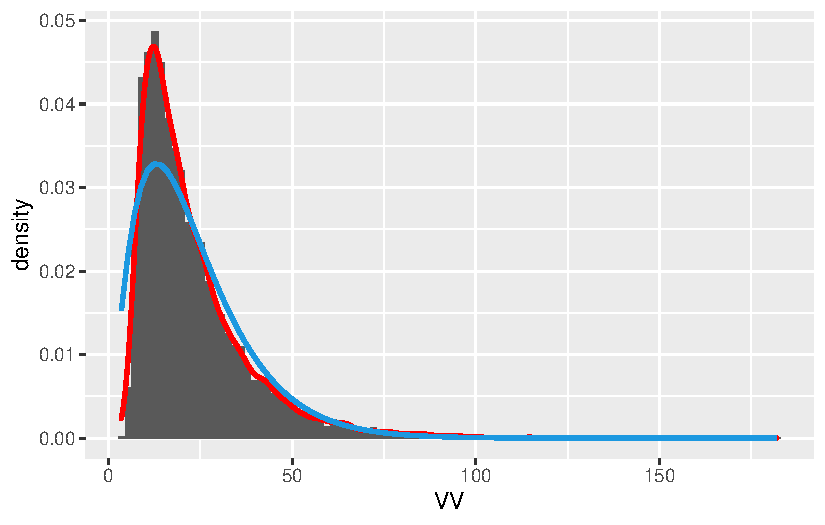
\includegraphics{Cinetique_Proteines_files/figure-pdf/approx density-1.pdf}

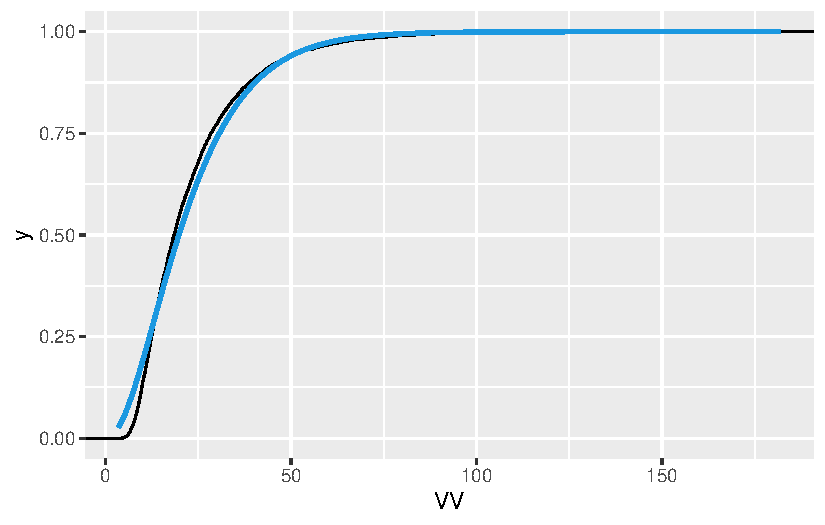
\includegraphics{Cinetique_Proteines_files/figure-pdf/approx repat-1.pdf}



\end{document}
